\documentclass[lettersize,journal]{IEEEtran}
\usepackage{amsmath,amsfonts}
\usepackage{algorithmic}
\usepackage{algorithm}
\usepackage{array}
\usepackage[caption=false,font=normalsize,labelfont=sf,textfont=sf]{subfig}
\usepackage{textcomp}
\usepackage{stfloats}
\usepackage{url}
\usepackage{verbatim}
\usepackage{graphicx}
\usepackage{cite}
\usepackage{BookTabs}
\usepackage{siunitx}
\usepackage{gensymb}
\usepackage{setspace}
\doublespacing
\hyphenation{op-tical net-works semi-conduc-tor IEEE-Xplore}
% updated with editorial comments 8/9/2021

\begin{document}
	
	\title{Pycnometry and Continuous Distillation of Ethanol-Water mixtures}
	
	\author{Joseph Zimmerman}
	% <-this % stops a space
	
	
	
	\maketitle
	
	\begin{abstract}
		In this paper, two experiments were conducted on ethanol-water mixtures. A pycnometer and quartz-tubed densitometer were used to determine liquid densities across a variety of compositions of ethanol and water. Alcohol-gauging tables from the US Alcohol and Tobacco Tax and Trade Bureau (TTB) were used to correlate theoretical densities of various compositions of ethanol and water at various temperatures to apparent proofs at 60F and finally correct to true proof and mole fraction of ethanol. Densities, measured through the pycnometer and densitometer, were compared. 
	\end{abstract}
	
	\begin{IEEEkeywords}
		Article submission, IEEE, IEEEtran, journal, \LaTeX, paper, template, typesetting.
	\end{IEEEkeywords}
	
	\section{Introduction}
	\IEEEPARstart{P}{ycnometry} is a fundamental laboratory technique used to determine the density of solid or liquid substances by measuring their mass and volume and comparing them to a known volume. A pycnometer—a calibrated glass flask with a defined volume—is filled with the sample, and its mass is compared to the mass of the same flask filled with a reference fluid (water in our case). Digital densitometers can also be used to determine the density of a solution. Our digital densitometer measures density through a vibrating "U-Tube". The sample is introduced into a U-shaped borosilicate glass tube that is being excited to vibrate at its characteristic frequency electronically. The characteristic frequency changes depending on the density of the sample. Through determination of the characteristic frequency the density of the sample can be calculated. In the first part of our experiment, we determined the densities of various compositions of ethanol-water through pycnometry and a digital densitometer. Alcohol-gauging tables from the US Alcohol and Tobacco Tax and Trade Bureau (TTB) were used to correlate theoretical densities of various compositions ranging from pure ethanol to pure water at various temperatures to apparent proofs at 60F and finally correct to extract true proof and mole fraction of ethanol.
	\newline
	\newline
	\-\hspace{0.6cm}This theoretical array of densities and corresponding mole fractions were then used in the second part of the lab, where we performed a continuous distillation of an ethanol-water mixture at two different reflux ratios, 4 and 5 in our case. 
	
	\section{Theory}
	\subsection{Pycnometry}
	The pycnometer used in our experiment was a Kimble KiMax pycnometer. By measuring the mass of the empty pycnometer, the mass of the pycnometer filled with water (our reference fluid), the known density of water, and the mass of the pycnometer filled with the experimental solution, the density of the experimental solution can be determined by \cite{ref1}. 
	\begin{equation}
		\label{deqn_ex1}
		V = \frac{m_{w}-m_{e}}{\rho_{water}(t)} = \frac{m_{sample}-m_{e}}{\rho_{sample}}
	\end{equation}
	where $m_{w}$ is the mass of the pycnometer filled with water, $m_{e}$ is the mass of the empty pycnometer, $\rho_{water}(t)$ is the density of water at temperature T, and $\rho_{sample}$ is the density of the sample at T. This equation can be arranged to solve for $\rho_{sample}$.
	\begin{equation}
		\label{deqn_ex2}
		\rho_{sample}  = \frac{m_{sample} - m_{empty}}{m_{water}-m_{sample}}\cdot\rho_{water}(T)
	\end{equation}
	
	\subsection{Gauging alcohol with TTB tables}
	Table 6 from the TTB correlates specific gravities of ethanol-water mixtures at 60$\degree$ F to proofs. In order to obtain proofs at other temperatures, one must convert the measured density ($\rho_{1}$) at a given temperature (T1) to the hypothetical density ($\rho_{2}$) that a glass hydrometer would indicate if calibrated at the standard 60$\degree F$ reference temperature:
	
	\begin{equation}
		\label{deqn_ex3}
		\rho_{2} = \rho_{1} (1 + \alpha(T_{1} - 60\degree F))
	\end{equation}
	where $\alpha$ is the coefficient of thermal expansion for the hydrometer material (typically 25 $\cdot$ $\frac{10\textsuperscript{-6}}{\degree C}$ for glass).
	At this corrected density, specific gravity can be calculated using the reference density of water at 60, $\degree C$ 0.99904 g/cc. Then, Table 6 can be interpolated through a truncated Taylor series expansion to retrieve an apparent proof, $C_{2}$, implemented as equation 1 in python:
	 
	\begin{equation}
		\label{deqn_ex4}
		C_{2} = f(\gamma_{1},T1) = [f + (\gamma_{1}-\gamma_{R})\frac{\partial f}{\partial \gamma} ] 
	\end{equation}
	where $\gamma_{1}$ is the specific gravity of the sample corrected to 60$\degree F$
	This apparent proof still has instrument and sample temperature effects, so it must be corrected to a true proof using TTB Table 1. The computed apparent proof $C_{2}$ is rounded down to the nearest integer and used as a reference for interpolation of Table 1.
	\begin{equation}
		\label{deqn_ex5}
		C_3 = C_2 + (C_2 - C_R) \frac{\partial f}{\partial C}\bigg|_{C_R, T_R} + (T_1 - T_R) \frac{\partial C}{\partial T}\bigg|_{C_R, T_R}
	\end{equation}
	where $C_{3}$ is the estimated true proof of the mixture corrected for temperature, $T_{1}$. $C_{R}$ and $T_{R}$ are reference proofs and temperatures from values corresponding to the rounded-down $C_{2}$ in Table 1.
	
	\subsection{Error Propagation}
	\subsubsection{Pycnometer Masses}
	 Uncertainty for each of the 10 mixtures in the pycnometer, the pure water in the pycnometer, and the empty pycnometer were calculated on a 95\% Confidence Interval (N=3). 
	\subsubsection{Pycnometer Densities}
	Uncertainties for the mixture densities determined with the pycnometer propogates from uncertainties in mass measurements. The standard formula for error propagation was applied to equation (2)
	\begin{equation}
		\label{deqn_ex6}
		\delta d_{f} = \sqrt{
			\begin{aligned}
				&\left(\frac{\partial d_{f}}{\partial m_{f}}\delta m_{f}\right)^2 + 
				\left(\frac{\partial d_{f}}{\partial m_{e}}\delta m_{e}\right)^2 \\
				&+ \left(\frac{\partial d_{f}}{\partial m_{w}}\delta m_{w}\right)^2 + 
				\left(\frac{\partial d_{f}}{\partial T}\delta T\right)^2
			\end{aligned}
		}
	\end{equation}
	where $\delta d_{f}$ is the uncertainty associated with the computed density, $\delta m_{f}$ is the uncertainty associated with the sample-filled pycnometer mass measurements, $\delta m_{e}$ is the uncertainty associated with the empty pycnometer mass measurements, and $\delta m_{w}$ is the uncertainty associated with the water-filled pycnometer mass measurements and the partial with respect to temperature is estimated with finite differences  
	\subsection{Distillation}
	\subsubsection{Vapor Liquid Equilibria}
	The theoretical stages of our distillation column are assumed to be at vapor-liquid equilibrium (VLE). The VLE behavior of ethanol and water can be modeled using Antoine's equation for determining saturation pressures, and the Van Laar model for activity-coefficients.
	First, the activity coefficients, $\gamma$, are calculated
	\begin{equation}
		\label{deqn_ex5.5}
		\gamma_{1} = A_{12}(\frac{A_{21}X_{2}}{A_{12}X_{1}+A_{21}X_{2}})^{2}
	\end{equation}
	\begin{equation}
		\label{deqn_ex5.5}
		\gamma_{2} = A_{21}(\frac{A_{12}X_{1}}{A_{12}X_{1}+A_{21}X_{2}})^{2}
	\end{equation}
	where $A_{12}$ and $A_{21}$ are Van Laar parameters for water and ethanol respectively. $X_{1}$ is the mole fraction of ethanol in solution and $X_{2}$ is the mole fraction of water.
	The Antoine Equation is used to determine saturation pressures of the pure components in the solutions and follows the form:
	\begin{equation}
		\label{deqn_ex5.5}
		log_{10}P^{*} = A - \frac{B}{T+C}
	\end{equation}
	where $P^{*}$ is the saturation pressure of the component and A, B, and C are tabulated constants.
	The VLE can then be modeled through the modified Raoult's Law:
	\begin{equation}
		\label{deqn_ex5.5}
		\gamma_{1}xP^{etOH*} = yP
	\end{equation}
	\begin{equation}
		\label{deqn_ex5.5}
		\gamma_{2}(1-x)P^{H2O*} = (1-y)P
	\end{equation}
	A solver like SciPy optimize's root function can be used to solve for saturation temperatures at a given pressure and a $T_{xy}$ diagram can be constructed
	\subsubsection{McCabe-Thiele diagram}
	McCabe-Thiele analysis is based on the McCabe-Thiele assumption: that liquid is vaporized at the same rate vapor is condensed on a molar basis. With this assumption, two mole balances can be constructed: one for the operating (rectifying) line and one for the stripping line. These lines will be plotted against the $T_{xy}$ equilibrium curve described earlier. The operating line passes through the point ($x_{p},x_{p}$), where $x_{p}$ is the product ethanol mol fraction, and follows the equation:
	\begin{equation}
		\label{deqn_ex5.5}
		y_{i} = \frac{O}{O+1}x_{i-1} + \frac{x_{p}}{O+1}
	\end{equation}
	Where O is the reflux ratio of the column. The stripping line passes through the point ($x_{w},x_{w}$), where $x_{w}$ is the waste ethanol mol fraction, and follows the equation:
	\begin{equation}
		\label{deqn_ex5.5}
		y_{i} = \frac{O+F}{O+1}x_{i-1} + \frac{1-F}{O+1}x_{W}
	\end{equation}
	Where F is the total molar flux per mole product.
	A feed line, often called 'q' or 'feed quality' line can then be drawn, intersecting at the feed composition on the X=Y line, with a slope determined by the enthalpy of the feed stream. 
	\begin{equation}
		\label{deqn_ex5.5}
		q = \frac{H_{F} - H_{L}}{H_{V} - H_{L}}
	\end{equation}
	where $H_{F}$ is the enthalpy of the feed stream at feed conditions, $H_{L}$ is the enthalpy of the feed stream at saturated liquid conditions, and $H_{V}$ is the enthalpy of the feed stream at saturated vapor conditions. We assume that the feed stream is entirely saturated liquid at steady state and thus q = 1.
	Straight lines can then be traced from the product composition, horizontally to the bubble point, then vertically until reaching the rectifying line, then repeated until reaching the bubble point of the stripping section. Then, the vertical lines will be drawn until the stripping line, in a similar fashion. Once a horizontal line passes the waste stream composition, stop.
	
	
	The overall column efficiency can then be calculated by
	\begin{equation}
		\label{deqn_ex5.5}
		E_{Column} = \frac{N_{theoretical}}{9}
	\end{equation}
	Where 9 comes from the 8 trays of the column, plus the reboiler stage.
	
	Theoretical compositions of trays can be computed by solving for mole fraction values with our VLE data given steady state tray temperatures.
	\subsubsection{Economic Analysis of Distillation}
	We can determine the economic efficiency of our batch distillation by comparing the commercial prices per kilogram of ethanol to our cost per kilogram determined by heater and condenser power draw and distillation time.
	The power of the condenser can be calculated by
	\begin{equation}
		\label{deqn_ex5.5}
		P [Watts] = I[Amps]V[Volts]
	\end{equation}
	Where V is the voltage of the condenser, measured by a meter at the power outlet, and I is 25A, for the Armfield UOP3BM-B.
	The total energy expended can be calculated as
	\begin{equation}
		\label{deqn_ex5.5}
		E {tot} = (P_{condenser} + P_{heater})t
	\end{equation}
	where t is the time of the distillation, in hours.
	
	According to the CA Public Utility Commission's Electric Rate Comparison tool, the average price per kilowatt-hour is 42 cents. Using this, the cost of our distillation can be computed.
	\begin{equation}
		\label{deqn_ex5.5}
		Cost= \frac{\$0.42}{kWh}E {tot} 
	\end{equation}
	The total mass of ethanol in the reflux stream can be determined by determining the proof (and thus ABV) of the product with our equations from the pycnometry experiment to get the volume of pure ethanol in the product stream, then multiplying by the density of pure ethanol.
	\begin{equation}
		\label{deqn_ex5.5}
		m_{Ethanol}= \rho_{ethanol}V_{product}ABV
	\end{equation}
	The energy cost per kilogram can then be computed by dividing the total cost of the distillation by the mass of ethanol produced during the distillation in kilograms
	
	\section{Experimental Methods}
	\subsection{Pycnometry}
	\begin{figure}[!t]
		\centering
		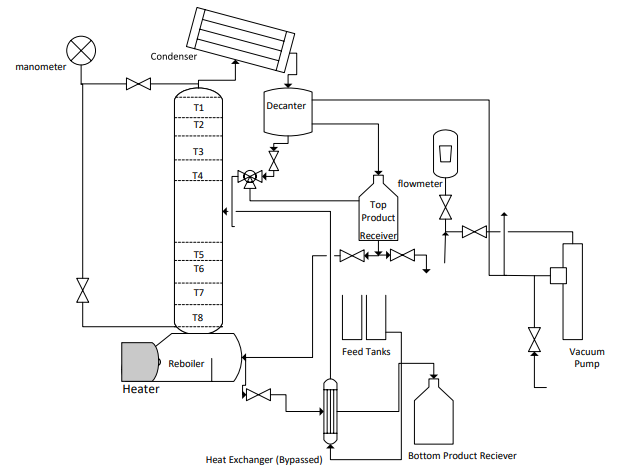
\includegraphics[width=3.6in]{Drawing}
		\caption{Schematic of the experimental distillation configuration. T1-8 are trays, horizontal plates to facilitate vapor-liquid contact and mass transfer of ascending vapor or descending liquid streams. The feed pump delivers feed to the column at a constant speed. The heater-powered reboiler serves as an energy source to vaporize the feed and reflux streams. Electrical energy is converted to heat by the heater. The condenser serves as a heat exchanger to condense vapor rising from the top of the column by dropping the temperature of the vapor stream. It is supplied with cooling water as well to the jacket.The reflux valve is electronically controlled and controls the divertion of the decanted stream from the top product receiver back into the column at intervals based on the reflux ratio of the column. The manometer is used to measure the pressure differential between the top and bottom of the distillation column. It is only active when both adjacent valves are open.}
		\label{fig_2}
	\end{figure}
	\subsubsection{Pycnometer Calibration}
	The pycnometer was rinsed thoroughly with ethanol and dried with compressed air. The mass of the empty (stopped and capped) pycnometer was weighed 3 times with an analytical balance and recorded as $M_{e}$. 
	The pycnometer was emptied, cleaned following the above procedure, and filled with deionized water (DIW). The mass of the water-filled pycnometer was weighed 3 times with an analytical balance and recorded as $M_{w}$ Then, 3 readings of density and temperature were taken with the densitometer and recorded as $\rho_{w}$
	\subsubsection{Pycnometer Sample Measurements}
	The pycnometer was emptied, rinsed thoroughly with ethanol and dried with compressed air. 10 ethanol-water mixtures ranging from pure ethanol to pure water were constructed. Various weights of ethanol and water were measured over 3 trials then combined in a beaker to form the samples we measured, cleaning the beaker and pycnometer before switching concentrations. The mass of the empty (stopped and capped) pycnometer was weighed 3 times with an analytical balance and recorded as $M_{e}$ Then, 3 readings of density and temperature were taken at every concentration with the densitometer and recorded as $\rho_{d_N}$.
	\subsection{Continuous Distillation}
	The distillation system used in this lab was the Armfield UOP3. Figure 1 is a schematic for the experimental setup. The reboiler power was set to 0.75kW, and the feed pump dial read '5.2', which can be corrected to a mL/s flowrate through a calibration equation. The column was initially ran in open reflux to reach operating temperature quickly without producing waste. Then, the reflux ratio was swapped to 4 (product flows to the top product receiver for 7 seconds, and back to the column for 28 seconds).  Waste and product was then drained from the top and bottom receivers in three, 1 minute trials. Three measurements were taken of the waste and product density with a densitometer, and weighed on an analytical balance. The weights of  waste and product streams were used to determine steady-state operation through mass balance closure. At steady state, samples were drawn from plates 2,4,6 and 8, and the densities were measured three times. At steady state, the condenser voltage draw was noted to be 117.9V.
	This procedure was repeated the following week at a reflux ratio of 5 (product flows to the top product receiver for 7 seconds, and back to the column for 35 seconds) At steady state, the condenser voltage draw was noted to be 118.5V.
	\section{Results}
	\subsubsection{Pycnometry and Theoretical Conversions from Density}
	The densities of the densitometer were consistently greater than the computed pycnometer densities, as shown by figure 4. There is significantly greater error associated with the pycnometer densities than the densitometer densities.
	
	\begin{figure}[!t]
		\centering
		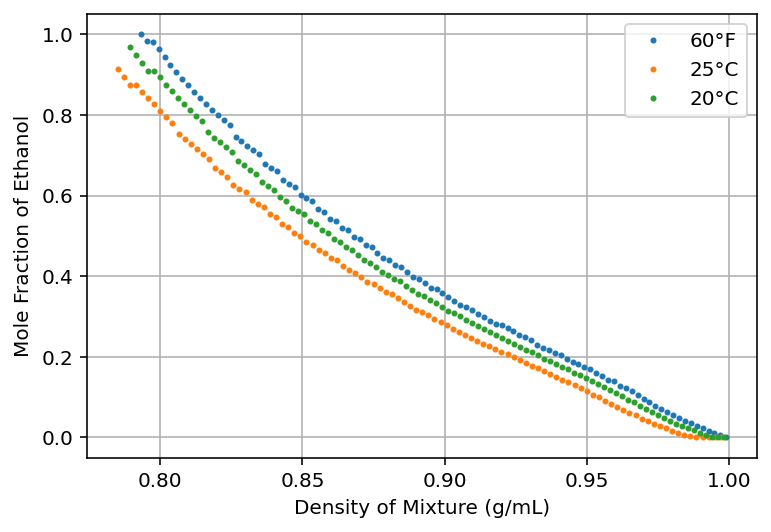
\includegraphics[width=3.6in]{fig1}
		\caption{ Mole fractions of theoretical ethanol-water mixtures ranging from pure ethanol to pure water calculated from interpolation of TTB alcohol proofing tables at various industry-standard temperature values. }
		\label{fig_1}
	\end{figure}
	% Reflux 4
	\begin{figure}[!t]
		\centering
		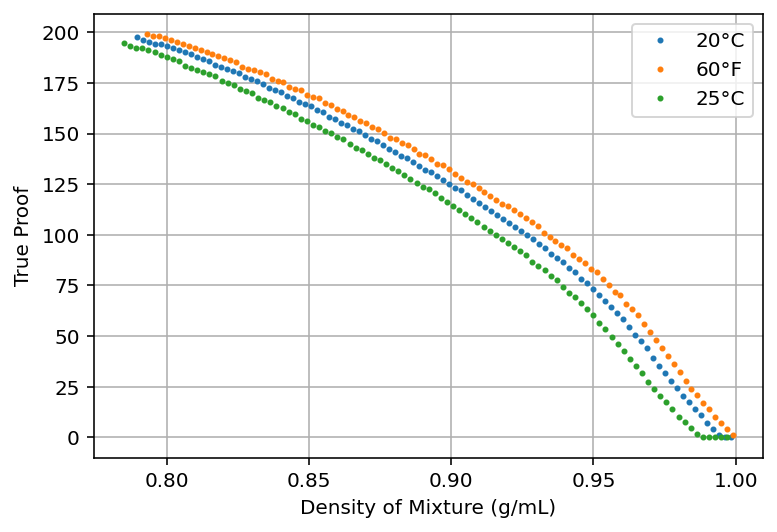
\includegraphics[width=3.6in]{fig2}
		\caption{{ True proofs of theoretical ethanol-water mixtures ranging from pure ethanol to pure water calculated from interpolation of TTB alcohol proofing tables at various industry-standard temperature values. } }
		\label{fig_2}
	\end{figure}
	\begin{table}[htbp]
		\centering
		\caption{Comparison of pycnometer densities corrected to 60\degree F with theoretical densities}
		\label{tab:density_results}
		\small
		\begin{tabular}{@{}c S[table-format=1.4]@{\,±\,}S[table-format=1.4] S[table-format=1.4] S[table-format=+1.2]@{}}
			\toprule
			\textbf{Sample} & \multicolumn{2}{c}{\textbf{Theoretical (g/mL)}} & \textbf{Experimental (g/mL)} & \textbf{\% Dev.} \\
			\midrule
			1  & 0.9270 & 0.0001 & 0.9277 & +0.08 \\
			2  & 0.8540 & 0.0001 & 0.8534 & -0.07 \\
			3  & 0.9322 & 0.0001 & 0.9319 & -0.03 \\
			4  & 0.9623 & 0.0001 & 0.9625 & +0.02 \\
			5  & 0.9713 & 0.0001 & 0.9716 & +0.03 \\
			6  & 0.8269 & 0.0001 & 0.8274 & +0.06 \\
			7  & 0.8718 & 0.0001 & 0.8716 & -0.02 \\
			8  & 0.9007 & 0.0001 & 0.9009 & +0.02 \\
			9  & 0.7937 & 0.0001 & 0.7842 & -1.20 \\
			10 & 0.9282 & 0.0001 & 0.9280 & -0.02 \\
			\bottomrule
		\end{tabular}
		
	\end{table}
	
	
	
	\begin{figure}[!t]
		\centering
		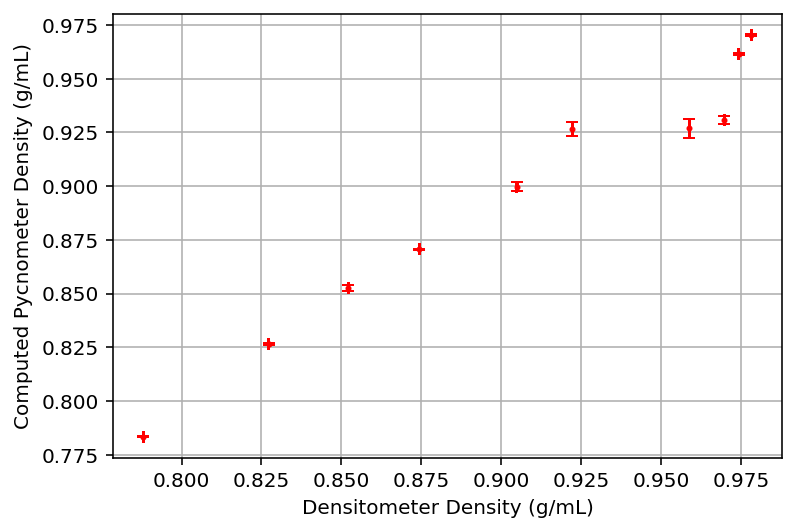
\includegraphics[width=3.6in]{fig3}
		\caption{Experimental ethanol-water mixture densities computed through pycnometry plotted against densitometer readings. Error bars for the y-axis, or pycnometer-derived densities, were derived from equation 6. Error bars for the x-axis were computed based on a 95\% confidence interval (N=3) }
		\label{fig_2}
	\end{figure}
	\subsubsection{Continuous Distillation}
	At steady state for reflux 4, the tray temperatures for Trays 2,4,6 and 8 were 79.0$\pm$0.1$\degree C$,80.1$\pm$0.2$\degree C$,86.0$\pm$0.2$\degree C$,	and 87.1$\pm$0.2$\degree C$, respectively.
	At steady state for reflux 5, the tray temperatures for Trays 1-8 were 78.7$\pm$0.1$\degree C$,80.1$\pm$0.3$\degree C$,86.0$\pm$0.4$\degree C$,	and 87.8$\pm$0.5$\degree C$, respectively. 
		\begin{table}[htbp]
			\centering
			\footnotesize
			\caption{Mass Balance Results at Different Reflux Ratios}
			\label{tab:mass_balance}
			\sisetup{
				separate-uncertainty,
				table-number-alignment = center,
				table-figures-uncertainty = 2,
				table-format = -1.2
			}
			\begin{tabular}{@{} l 
					S[table-format=3.2(1)]  % Mass In
					S[table-format=3.1(3)]  % Mass Out (fixed uncertainty width)
					S[table-format=-1.2]    % Deviation
					@{}}
				\toprule
				\textbf{Reflux} & 
				\textbf{Mass In} & 
				\textbf{Mass Out} & 
				\textbf{\% Dev.} \\
				& \textbf{(g/min)} & \textbf{(g/min)} & \\
				\midrule
				Reflux 5:1 & 53.90 \pm 0.10  & 59.0 \pm 12.3  & -9.32 \\
				Reflux 4:1 & 56.60 \pm 0.05  & 74.2 \pm 120   & -31.01 \\
				\bottomrule
			\end{tabular}
		\end{table}
		The mass balance for the reflux ratio of 5 closed within 10\%, but the reflux ratio of 4 balance did not. There was high uncertainty associated with the waste stream of this ratio, which affected the mass out uncertainty. 
		
		

	
	
	
		
	
	\begin{figure}[!t]
		\centering
		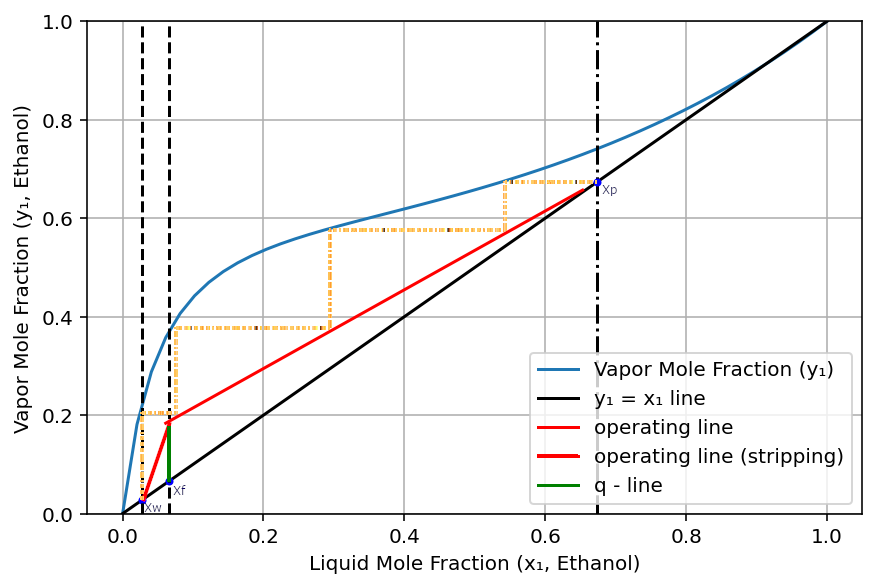
\includegraphics[width=3.6in]{reflux4}
		\caption{McCabe-Thiele diagram of the distillation column ran at a reflux ratio of 4 (28 seconds overhead feed to column, 7 seconds to the top product receiver). The yellow horizontal lines represent theoretical stages, while the yellow vertical lines correspond to the VLE conditions of the theoretical stage.The product mole fraction of ethanol, $X_{p}$, feed mole fraction of ethanol, $X_{f}$, and waste mole fraction of ethanol, $X_{w}$ were 0.67,0.07 and 0.03, respectively The feed pump was operated at a flow rate of 58.1 $\frac{mL}{min}$. The pressure drop across the column was measured as 90.0mm $H_{2}O$ through the manometer. The heater power was 0.75kW, while the condenser operated at 3.0kW.} 
		\label{fig_2}
	\end{figure}
	\begin{figure}[!t]
		\centering
		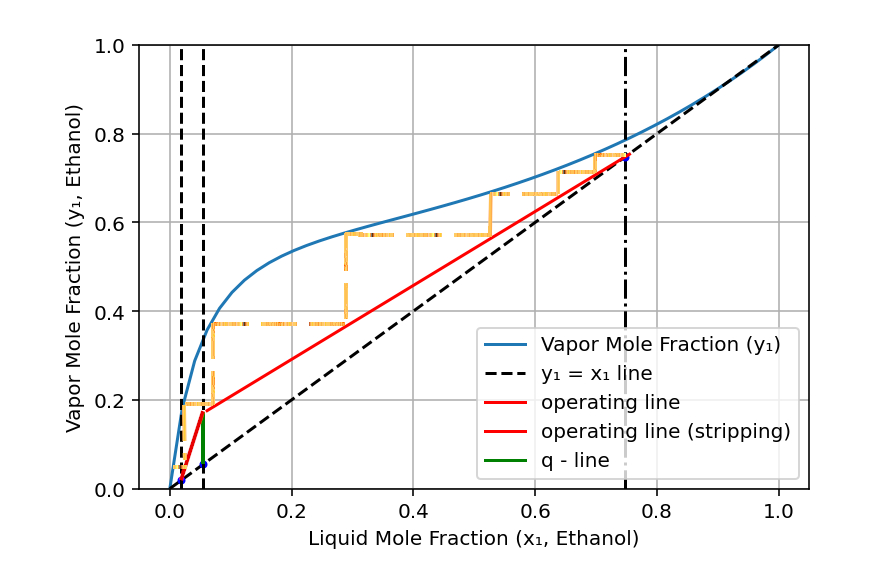
\includegraphics[width=3.6in]{reflux5}
		\caption{McCabe-Thiele diagram of the distillation column ran at a reflux ratio of 5 (35 seconds overhead feed to column, 7 seconds to the top product receiver). The yellow horizontal lines represent theoretical stages, while the yellow vertical lines correspond to the VLE conditions of the theoretical stage. The product mole fraction of ethanol, $X_{p}$, feed mole fraction of ethanol, $X_{f}$, and waste mole fraction of ethanol, $X_{w}$ were 0.75,0.05 and 0.02, respectively. The feed pump was operated at a flow rate of 58.1 $\frac{mL}{min}$. The pressure drop across the column was measured as 94.5mm $H_{2}O$ through the manometer. The heater power was 0.75kW, while the condenser operated at 2.9kW.} 
		\label{fig_3}
	\end{figure}
	
	The overall column efficiency in the case of a reflux ratio of 4, as calculated by equation (15) was 0.44. For the reflux ratio of 5, it was calculated to be 0.66. The rectifying and stripping line for the reflux ratio of 4 was slightly steeper than that of reflux ratio 5. In both cases, the tray mole fractions deviated from theoretical values retrieved with theoretical VLE data and steady state tray temperatures. 
	
	
		
	\begin{table}[htbp]
		\centering
		\caption{Theoretical vs. Experimental Mole Fractions at Reflux 4}
		\label{tab:reflux4}
		\begin{tabular}{ccc}
			\toprule
			\textbf{Tray} & \textbf{Theoretical} & \textbf{Experimental} \\
			\midrule
			2 & 0.09 & 0.11 \\
			4 & 0.12 & 0.13 \\
			6 & 0.50 & 0.44 \\
			8 & 0.68 & 0.65 \\
			\bottomrule
		\end{tabular}
	\end{table}
		
	\begin{table}[htbp]
		\centering
		\caption{Theoretical vs. Experimental Mole Fractions at Reflux 5}
		\label{tab:reflux5}
		\begin{tabular}{ccc}
			\toprule
			\textbf{Tray} & \textbf{Theoretical} & \textbf{Experimental} \\
			\midrule
			2 & 0.08 & 0.09 \\
			4 & 0.12 & 0.12 \\
			6 & 0.50 & 0.45 \\
			8 & 0.75 & 0.66 \\
			\bottomrule
		\end{tabular}
	\end{table}
	\begin{table}[htbp]
		\centering
		\caption{Distillation Cost Comparison (\$/kg)}
		\label{tab:cost_compact}
		\begin{tabular}{l@{\hspace{4pt}}r@{\hspace{4pt}}r@{\hspace{4pt}}r}
			\toprule
			\textbf{Component} & \textbf{Reflux 4} & \textbf{Reflux 5} & \textbf{Commercial} \\
			\midrule
			Heater    & 32.40 & 21.59 & --- \\
			Condenser & 127.96 & 84.85 & --- \\
			\midrule
			Total     & 160.36 & 106.45 & 0.23 \\
			\bottomrule
		\end{tabular}
	\end{table}
	
		
	
	
	
	
	
	
	\section{Discussion}
\subsection{Temperature effect on density measurements}
\subsubsection{Temperature effects on Pycnometer readings and density}
As a fluid's temperature increases, it's volume increases due to thermal expansion. This changes the amount of mass that can fit in the pycnometer, but can be corrected for. We accounted for this by using the thermal expansion coefficient of the pycnometer material (glass) at a reference temperature of 60$\degree$F. This was incorporated into the true\_proof and pycnometer working equations in python. We accounted for the thermal expansion of the ethanol-water mixture by interpolation of TTB tables 1 and 6 for gauging alcohol, but a similar equation for thermal expansion could be used:
\begin{equation}
	\label{deqn_ex5.5}
	V_{T} = V_{o}[1+\alpha(T-T{o})]
\end{equation}
where $V_{T}$ is the volume of the fluid at temperature T, $V_{o}$ is the volume of the fluid at reference temperature $T_{o}$, and $\alpha$ is the coefficient of thermal expansion of the fluid
\subsubsection{Effect of temperature on mole fraction in ethanol-water mixtures}
Temperature has an effect on density so in calculating mole fraction from TTB tables which use specific gravity at a reference temperature, we must ensure we correct to the same reference temperature for accurate calculation. 
\subsection{Steady State Operation in Distillation Columns}
Steady state operation in a column was determined by verifying that the mass balance of the column reduces to $Mass_{in} = Mass_{out}$, as determined by weights of the waste and product streams and feedrate. Due to operational fluctuations, a 10\% range was considered acceptable.
\subsubsection{Mass balance error}
Fluctuations in the reboiler power could effect the mass balance by changing the column temperature and VLE behavior of the ethanol-water mixture, and were likely a large source of random error. This can be noted in the column data, where there were apparent deviations in the reboiler data. If one collects a sample for too short a duration of time, they could not capture a full reflux cycle (35s for reflux ratio of 4, 42s for reflux ratio of 5) and product/waste flowrates will be effected. This is a form of systemic error. In both cases, error can be minimized by collecting samples for an appropriate duration of time (1-5min)
\subsubsection{Variations of operational parameters on steady state}
Sudden variations in flowrate can change the composition of the product and waste compositions, as the mass balance of the system will be altered. The temperature profile of the trays would also be affected as the energy balance of the column is altered. Sudden variations in reboiler power will also alter the energy balance of the column and affect the temperature profiles of the trays. It will also lead to increased vapor generation which will affect the mass balance of the system.
Sudden variations in the reflux ratio will alter product and waste flowrates, altering the mass balance because different amounts of product will be returned to the column while the feed remains constant.
\subsection{Distillation Column Performance Analysis}
\subsubsection{McCabe-Thiele Analysis}
The McCabe-Thiele method of modeling distillation assumes that the distillation column operates at a constant pressure (isobaric), and with constant molal overflow. Constant molal overflow means that the number of moles of mixture vaporizing is equal to the moles of mixture condensing. With fluctuations in reboiler power, however, this was likely not the case for our experiment. The theoretical trays are typically significantly higher(as they were in our case) as they assume 100\% tray efficiency, with full seperation according to VLE data, but, in practice, efficiency is less than 100\% due to flooding, entrainment or incomplete mixing.
\subsubsection{Theoretical and Experimental VLE Data Comparison}
Differences between Theoretical and Experimental VLE data differ and depend on the model used for the theoretical VLE relationship; the interaction of components in binary mixtures varies widely depending on the substance and there are many equations of state suitable for different types of components. Water and ethanol notoriously form an azeotrope and model results can vary. This could potentially affect the theoretical tray calculation as determined by the McCabe-Thiele diagram. 

Thermodynamic parameters like activity coefficients, fugacity and equilibrium constants are used to describe the behaviors of mixtures and components in them. Theoretical VLE models like Val-Laar, NRTL, and Wilson use published values from experimental data to model solution behavior.
\subsection{Improvements to Experiment Design}
\subsubsection{Pycnometry}
A big concern during the pycnometry experiment was the presence of air bubbles in the solution. After pouring the sample inside, there were often lots of tiny bubbles along the inside surfaces of the flask. This would displace volume that could otherwise be occupied by sample mixture, and could lead to inaccurate densitometer readings if bubbles are drawn into the device. We tried to mediate this by letting samples sit for ~2-3minutes and by tapping the sides of the flask with it uncapped, but some bubbles nonetheless persisted. A potential fix for this would be some form of ultrasonic agitation, to agitate bubbles to the surface of the fluid, or a vacuum apparatus to pull off air bubbles before measurements are taken.
\subsubsection{Continuous Distillation}
In our McCabe-Thiele diagrams, we make an assumption that the feed stream is entirely saturated vapor. The stripping line was graphically fitted between the intersection of the x-y line and the intersection of the q and rectifying line, so by relaxing this assumption and accounting for feed quality, the stripping line will be altered. If the feed is cold, for instance, the slope of the q line will be greater than 1, and the distillation will have more stripping sections due to the rectifying line and q line occurring further downfield. A way to monitor feed quality , such as a temperature and pressure sensor paired with VLE data in the feed to the column, could be used to more accurately determine feed quality. With a better estimate for q, one can choose an optimal entrance stage for the feed based on the new McCabe-Thiele modeling. 
One may consider swapping the trays for a packing material, like Dupont Hypak, which typically have lower height-equivalent to theoretical plate (HETP)  values than trays. This will decrease the length of the column, decreasing the pressure drop, reducing energy needs.
As the economic efficiency of the higher reflux ratio in terms of cost per kg of ethanol produced was better than that of the lower reflux ratio, it would be worthwhile to run further experiments at higher reflux ratios until the energy costs become too significant, optimizing for a maximum cost per kilogram.
\subsubsection{VLE}
The relationship between experimental and theoretical VLE behavior can be refined by 

\section{Technical Advances}





\section{References Section}
You can use a bibliography generated by BibTeX as a .bbl file.
BibTeX documentation can be easily obtained at:
http://mirror.ctan.org/biblio/bibtex/contrib/doc/
The IEEEtran BibTeX style support page is:
http://www.michaelshell.org/tex/ieeetran/bibtex/

% argument is your BibTeX string definitions and bibliography database(s)
%\bibliography{IEEEabrv,../bib/paper}
%
\section{Simple References}
You can manually copy in the resultant .bbl file and set second argument of $\backslash${\tt{begin}} to the number of references
(used to reserve space for the reference number labels box).

\begin{thebibliography}{1}
	\bibliographystyle{IEEEtran}
	
	\bibitem{ref1}
	{\it{Mathematics Into Type}}. American Mathematical Society. [Online]. Available: https://www.ams.org/arc/styleguide/mit-2.pdf
	
	\bibitem{ref2}
	T. W. Chaundy, P. R. Barrett and C. Batey, {\it{The Printing of Mathematics}}. London, U.K., Oxford Univ. Press, 1954.
	
	\bibitem{ref3}
	F. Mittelbach and M. Goossens, {\it{The \LaTeX Companion}}, 2nd ed. Boston, MA, USA: Pearson, 2004.
	
	\bibitem{ref4}
	G. Gr\"atzer, {\it{More Math Into LaTeX}}, New York, NY, USA: Springer, 2007.
	
	\bibitem{ref5}M. Letourneau and J. W. Sharp, {\it{AMS-StyleGuide-online.pdf,}} American Mathematical Society, Providence, RI, USA, [Online]. Available: http://www.ams.org/arc/styleguide/index.html
	
	\bibitem{ref6}
	H. Sira-Ramirez, ``On the sliding mode control of nonlinear systems,'' \textit{Syst. Control Lett.}, vol. 19, pp. 303--312, 1992.
	
	\bibitem{ref7}
	A. Levant, ``Exact differentiation of signals with unbounded higher derivatives,''  in \textit{Proc. 45th IEEE Conf. Decis.
		Control}, San Diego, CA, USA, 2006, pp. 5585--5590. DOI: 10.1109/CDC.2006.377165.
	
	\bibitem{ref8}
	M. Fliess, C. Join, and H. Sira-Ramirez, ``Non-linear estimation is easy,'' \textit{Int. J. Model., Ident. Control}, vol. 4, no. 1, pp. 12--27, 2008.
	
	\bibitem{ref9}
	R. Ortega, A. Astolfi, G. Bastin, and H. Rodriguez, ``Stabilization of food-chain systems using a port-controlled Hamiltonian description,'' in \textit{Proc. Amer. Control Conf.}, Chicago, IL, USA,
	2000, pp. 2245--2249.
	
\end{thebibliography}


\newpage

\section{Biography Section}
If you have an EPS/PDF photo (graphicx package needed), extra braces are
needed around the contents of the optional argument to biography to prevent
the LaTeX parser from getting confused when it sees the complicated
$\backslash${\tt{includegraphics}} command within an optional argument. (You can create
your own custom macro containing the $\backslash${\tt{includegraphics}} command to make things
simpler here.)

\vspace{11pt}

\bf{If you include a photo:}\vspace{-33pt}
\begin{IEEEbiography}[{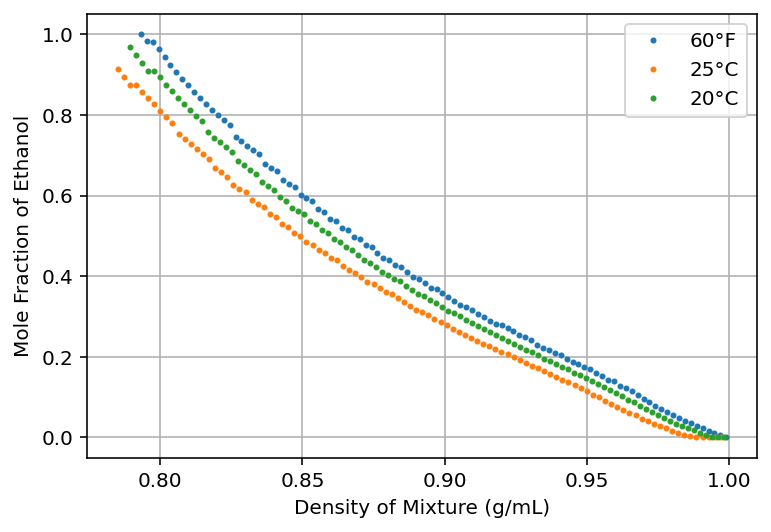
\includegraphics[width=1in,height=1.25in,clip,keepaspectratio]{fig1}}]{Michael Shell}
	Use $\backslash${\tt{begin\{IEEEbiography\}}} and then for the 1st argument use $\backslash${\tt{includegraphics}} to declare and link the author photo.
	Use the author name as the 3rd argument followed by the biography text.
\end{IEEEbiography}

\vspace{11pt}

\bf{If you will not include a photo:}\vspace{-33pt}
\begin{IEEEbiographynophoto}{John Doe}
	Use $\backslash${\tt{begin\{IEEEbiographynophoto\}}} and the author name as the argument followed by the biography text.
\end{IEEEbiographynophoto}




\vfill

\end{document}
